\section{Results}
\label{sec:results}

\subsection{The grid as run}
\label{sec:compliance}

\paragraph{Scope.} Of the 18 cells, 16 were run on the registered configuration and form the grid of Table~\ref{tab:cells}. The registered build of \texttt{qwen3.5-4b} became unavailable before its retail cell ran; that cell was run on a later build of the same model, with its own SAS calibration, and is reported outside every fit (Appendix~\ref{app:local4b}). The airline \texttt{qwen3.5-4b} cell was not run by us; a collaborator's MAS run of it enters only as a sensitivity (Appendix~\ref{app:local4b}).

\paragraph{Cells below 45\%.} Two cells are clearly below 45\%, one straddles and thirteen are clearly above (Table~\ref{tab:cells}). The weakest open model, \texttt{qwen3.5-4b} served at 4-bit, scores 94.7\% on telecom, above every closed model (\texttt{qwen3.5-9b} scores 95.3\%), and adds no low cell. Telecom separates the models most: the two low-tier closed models sit at 32.7 and 34.0\%, \texttt{gpt-5-mini} at 77.3\%, and \texttt{gemini-3-flash} and both open models at 91.3 to 95.3\%. The principle's distinctive prediction, a gain below 45\%, is therefore tested on two cells.

\paragraph{Validity and one deviation from the plan.} The twelve OpenAI and Google MAS cells and telecom $\times$ \texttt{qwen3.5-4b} pass the four mechanical bars: calls cut, tokens in cut calls, turns with two cut calls outside the exhaustion turn, and JSON or cut text sent to the customer (Table~\ref{tab:validity}). The fidelity bar was not met in any cell. Under the stricter of our two audits, which counts each unique order once and counts a refused order as not executed, write orders were executed exactly as issued in 9 to 41\% of cases per cell (680 of 2,744, 25\%, over the 13 cells): the orchestrator plans without the tool schemas, which only the database agent holds, so 13\% of its orders named a tool that does not exist and were mapped to the right one, 19\% carried argument names the tool does not take and were corrected, and 41\% were refused or diverted and reported back (Table~\ref{tab:validity}). The pre-registered response to a protocol failure is a bug-class fix and a re-run. The fix was implemented after the grid had been read: the orchestrator receives the tool definitions with tool choice disabled, so it still cannot call a tool. On a smoke of 5 tasks on each of three cells it raised the share of orders executed as issued from about 25\% to 72\% (13 of 18), short of the bar, with two of the five misses being refusals by the database agent on policy grounds, which no orchestrator-side change touches. The grid was not re-run. We therefore report the MAS as built and label this a deviation from the plan; throughout, ``the 13 cells'' means the 13 cells that meet the mechanical bars, and we read the unexecuted orders as part of what dividing the work costs in this architecture, which limits what the results say about designs that share tool schemas (\S\ref{sec:discussion}). \texttt{qwen3.5-4b} failed to parse 56\% of its plan calls; excluding its cell leaves the pattern of every result unchanged (sign match 9 of 11, binomial $p = 0.065$; pooled WW change $-0.7$ points, CI $[-2.9, +1.3]$). The three \texttt{qwen3.5-9b} cells fail the mechanical bars, all on turns with two cut calls and two on tokens in cut calls; a larger cap for one family would change the protocol, so they enter only a sensitivity. The \texttt{qwen3.5-4b} cell has no leave-one-domain-out index, so the primary fit uses 12 cells.

\begin{table}[t]
\caption{\textbf{No cell shows a MAS benefit.} The grid in the cost-bounded arm ($B = 4\Bx$, $c = \Bx$, $r = 4$; 150 episodes per system), \passone\ in percent with task-cluster bootstrap CIs. Exh.: MAS episodes ending budget exhausted; util.: median share of the ceiling spent; fin./exh.: pass rates of MAS episodes that finished and that were exhausted; tokens: median MAS completion tokens per episode over the SAS median (the ceiling bounds this ratio at $B$ over the SAS median, 5.0 to 6.3 across cells). $\dagger$: fails the mechanical bars, sensitivity only; SAS values computed by a collaborator. $\ddagger$: local route; per trial the MAS passed 15, 11 and 9 of 50, with the third trial affected by the route's fixed sampling seed (Appendix~\ref{app:local4b}).}
\label{tab:cells}
\begin{center}
\scriptsize
\setlength{\tabcolsep}{2.5pt}
\begin{tabular}{@{}llrlrlrrcr@{}}
\toprule
Model & Domain & SAS & SAS 95\% CI & MAS & Gain [95\% CI] & Exh. & Util. & Fin./exh. & Tokens \\
\midrule
\texttt{gpt-5-nano} & airline & 42.7 & [31.3, 54.0]$^{\circ}$ & 45.3 & $+2.7$ [$-6.7$, $+12.7$] & 23\% & 0.50 & 50\% / 31\% & 2.9$\times$ \\
 & retail & 68.0 & [58.7, 77.3] & 44.7 & $-23.3$ [$-32.7$, $-13.3$] & 16\% & 0.63 & 52\% / 8\% & 3.1$\times$ \\
 & telecom & 32.7 & [22.7, 43.3]$^{\downarrow}$ & 19.3 & $-13.3$ [$-20.7$, $-6.0$] & 15\% & 0.54 & 20\% / 13\% & 2.8$\times$ \\
\addlinespace[2pt]
\texttt{gpt-5-mini} & airline & 74.7 & [64.7, 84.0] & 58.0 & $-16.7$ [$-27.3$, $-6.7$] & 34\% & 0.83 & 68\% / 39\% & 5.2$\times$ \\
 & retail & 76.0 & [66.7, 84.0] & 48.0 & $-28.0$ [$-40.0$, $-17.3$] & 43\% & 0.90 & 68\% / 22\% & 4.9$\times$ \\
 & telecom & 77.3 & [68.0, 86.0] & 66.0 & $-11.3$ [$-18.7$, $-4.0$] & 18\% & 0.70 & 79\% / 7\% & 4.2$\times$ \\
\addlinespace[2pt]
\texttt{gemini-3.1-flash-lite} & airline & 78.7 & [68.0, 88.7] & 62.7 & $-16.0$ [$-24.0$, $-8.0$] & 31\% & 0.71 & 85\% / 13\% & 4.1$\times$ \\
 & retail & 77.3 & [67.3, 86.7] & 41.3 & $-36.0$ [$-47.3$, $-24.0$] & 58\% & 1.00 & 75\% / 17\% & 5.2$\times$ \\
 & telecom & 34.0 & [24.0, 44.7]$^{\downarrow}$ & 12.0 & $-22.0$ [$-30.7$, $-12.7$] & 45\% & 0.96 & 20\% / 1\% & 5.8$\times$ \\
\addlinespace[2pt]
\texttt{gemini-3-flash} & airline & 80.7 & [70.7, 90.0] & 55.3 & $-25.3$ [$-36.7$, $-14.0$] & 51\% & 1.00 & 74\% / 37\% & 6.1$\times$ \\
 & retail & 80.0 & [70.7, 88.7] & 25.3 & $-54.7$ [$-66.0$, $-44.0$] & 67\% & 1.00 & 63\% / 7\% & 5.1$\times$ \\
 & telecom & 91.3 & [86.0, 96.0] & 10.7 & $-80.7$ [$-87.3$, $-73.3$] & 68\% & 1.00 & 33\% / 0\% & 5.4$\times$ \\
\addlinespace[2pt]
\texttt{qwen3.5-4b}$^{\ddagger}$ & telecom & 94.7 & [90.7, 98.0] & 23.3 & $-71.3$ [$-80.0$, $-62.7$] & 63\% & 1.00 & 54\% / 5\% & 5.3$\times$ \\
\addlinespace[2pt]
\texttt{qwen3.5-9b}$^{\dagger}$ & airline & 79.3 & [71.3, 86.7] & 61.3 & $-18.0$ [$-28.7$, $-6.7$] & 12\% & -- & -- & -- \\
 & retail & 76.0 & [66.7, 84.7] & 49.3 & $-26.7$ (no paired CI) & 10\% & 0.51 & 55\% / 0\% & -- \\
 & telecom & 95.3 & [91.3, 98.7] & 33.3 & $-62.0$ (no paired CI) & 33\% & 0.93 & 48\% / 4\% & -- \\
\bottomrule
\multicolumn{10}{@{}l}{$^{\downarrow}$ SAS CI entirely below 45\%; $^{\circ}$ SAS CI straddles 45\%; every other cell is entirely above. Airline and retail \texttt{qwen3.5-4b}: Appendix~\ref{app:local4b}.}
\end{tabular}
\end{center}
\end{table}

\begin{table}[tbp]
\caption{G1 indicators per MAS cell at $4\times$, computed from logs. Bars: calls cut at the cap $\le 5\%$; tokens in cut calls $\le 10\%$; no turn with two or more cut calls outside the final exhaustion turn (shown as exhaustion / other); no JSON or cut text sent to the customer. Reported indicators: episodes (of 150) that consulted the advisor; plan calls that did not parse (share and count); forced customer messages; and the share of unique write orders executed exactly as issued under the stricter audit (a refused or diverted order counts as not executed). The fidelity bar ($\ge 90\%$ as issued) fails in every cell. Last column: whether the mechanical bars are met. ``--'': not available from the collaborator's files.}
\label{tab:validity}
\begin{center}
\scriptsize
\setlength{\tabcolsep}{3pt}
\resizebox{\linewidth}{!}{%
\begin{tabular}{@{}llccccrrrcl@{}}
\toprule
Model & Domain & Cut calls & Cut tokens & 2-cut (exh./other) & JSON/cut text & Advisor & Plan fail (n) & Forced & As issued & Bars \\
\midrule
\texttt{gpt-5-nano} & airline & 0.3\% & 0.3\% & 0 / 0 & 0 & 17 & 3.5\% (48) & 31 & 16\% & met \\
 & retail & 0.4\% & 0.5\% & 0 / 0 & 0 & 13 & 1.1\% (15) & 43 & 10\% & met \\
 & telecom & 0.3\% & 0.5\% & 0 / 0 & 0 & 9 & 1.6\% (30) & 51 & 20\% & met \\
\texttt{gpt-5-mini} & airline & 0.9\% & 0.9\% & 0 / 0 & 0 & 21 & 3.9\% (46) & 40 & 31\% & met \\
 & retail & 1.3\% & 1.4\% & 0 / 0 & 0 & 7 & 4.8\% (58) & 54 & 39\% & met \\
 & telecom & 0.5\% & 0.5\% & 0 / 0 & 0 & 8 & 1.9\% (32) & 25 & 41\% & met \\
\texttt{gemini-3.1-flash-lite} & airline & 1.8\% & 2.5\% & 0 / 0 & 0 & 93 & 3.7\% (37) & 38 & 13\% & met \\
 & retail & 3.5\% & 6.7\% & 2 / 0 & 0 & 106 & 6.6\% (68) & 78 & 13\% & met \\
 & telecom & 1.8\% & 2.0\% & 0 / 0 & 0 & 130 & 4.0\% (39) & 39 & 15\% & met \\
\texttt{gemini-3-flash} & airline & 1.9\% & 3.0\% & 1 / 0 & 0 & 147 & 4.9\% (48) & 46 & 41\% & met \\
 & retail & 3.3\% & 5.8\% & 1 / 0 & 0 & 150 & 5.2\% (46) & 42 & 19\% & met \\
 & telecom & 1.7\% & 1.5\% & 0 / 0 & 0$^{a}$ & 150 & 6.0\% (66) & 64 & 29\% & met \\
\texttt{qwen3.5-4b} & telecom & 2.3\% & 8.0\% & 0 / 0 & 0$^{a}$ & 14 & 56.2\% (1,386) & 1,076 & 9\% & met \\
\texttt{qwen3.5-4b}$^{c}$ & retail (Oct.\ build) & 3.6\% & 15.6\% & 7 / 5 & 0 & 13 & 21.3\% (347) & 80 & 16\% & fails \\
\texttt{qwen3.5-4b}$^{d}$ & airline (collab.) & 3.2\% & 12.9\% & 3 / 1 & 0 & 22 & 21.1\% (360) & 90 & 33\% & fails \\
\texttt{qwen3.5-9b} & airline$^{b}$ & -- & 35.7\% & 5 / 9 & 0 & -- & 33\% (492) & -- & -- & fails \\
 & retail & -- & 9.6\%$^{e}$ & 1 / 4 & 0 & 59 & 25\% (352) & 144 & -- & fails \\
 & telecom & 3.2\%$^{f}$ & 12.9\% & 5 / 6 & 0 & 52 & 14\% (292) & 122 & -- & fails \\
\bottomrule
\end{tabular}}
\end{center}
\vspace{2pt}
{\footnotesize\setlength{\parindent}{0pt} Notes. $^{a}$ One \texttt{cut text} flag raised by the checker, inspected and found to be a false positive: a plan call with \texttt{finish\_reason: length} and a complete JSON object; the customer message was complete. $^{b}$ Run by a collaborator on the same configuration at a later commit of the benchmark, outside the pinned commit's history. $^{c}$ Run on the October build of the model, outside every fit (Appendix~\ref{app:local4b}). $^{d}$ Run by a collaborator on the registered build against a budget calibrated on a SAS from a different serving stack; enters only as a sensitivity (Appendix~\ref{app:local4b}). Double cuts: the three non-zero entries among the 13 cells that meet the bars are all on exhaustion turns, which the amended bar allows (amendment adopted 17 October 2026, after the cells were read; no cell changes status under it). Write orders, stricter audit: 2,744 unique orders over the 13 cells; 24.8\% executed as issued; 13.1\% named a tool that does not exist and were mapped to the right one; 19.4\% carried argument names the tool does not take and were corrected; 41.1\% refused or diverted and reported back; 1.5\% executed with a changed value. $^{e}$ 13.2\% excluding runaway calls. $^{f}$ Share of plan calls. The looser audit of the plan (2,771 closed assignments, an order counted by what the database agent then executed) gives 28\% as issued, 36\% executed with a different tool or arguments, 35\% not executed, 0.6\% not verifiable. Fix smoke (orchestrator shown the tool definitions, tool choice disabled; 5 tasks on each of three cells, one trial): 13 of 18 orders as issued (1 of 4, 7 of 9, 5 of 5); the misses were two policy refusals by the database agent, one parallel-call wrapper, one customer-side tool and one corrected key.\par}
\end{table}

\paragraph{Read-call limit.} The database agent's limit of $r = 4$ was reached on 35 / 26 / 17\% of read orders (airline / retail / telecom) for \texttt{gemini-3.1-flash-lite}, 50 / 36 / 51\% for \texttt{gemini-3-flash}, 68 / 55 / 44\% for \texttt{gpt-5-mini} and 30 / 72\% for \texttt{gpt-5-nano} on retail / telecom, so it bound on 17 to 72\% of read orders in the 11 cells where it was counted. Re-running two telecom cells at $r = 25$ left both gains inside their $r = 4$ intervals ($-21.3$ against $-22.0$; $-77.3$ against $-80.7$) and plan calls per episode flat, so the overhead sits in the orchestrator's planning.

\paragraph{The hosted route of the 9-billion model.} The route returned more than \texttt{max\_tokens} on 17 (telecom) and 12 (retail) calls, of which 4 and 6 were runaway calls of about 131k reasoning tokens that exhausted the episode in one call, while the collaborator's retail replication had 6 such calls and no runaway, so the route's handling of the reasoning budget varies by run; \passone\ excluding those episodes is 34.2\% [27.0, 42.3] on telecom and 51.4\% [43.3, 59.4] on retail. Retail $\times$ \texttt{qwen3.5-9b} run twice with the same agent settings and budgets (ours at concurrency 4 on the pinned commit; the collaborator's at concurrency 1 on a later benchmark commit) gave 49.3\% and 51.3\%.

\subsection{The grid: no cell shows a MAS benefit}
\label{sec:grid}

Table~\ref{tab:cells} gives the grid before any regression. The MAS is below the SAS in 12 of the 13 cells, with a gain CI excluding zero in each, and ties in the straddling cell; the three cells that fail the mechanical bars show the same sign. Within families the loss grows with the strength of the SAS, and the largest losses fall on the two cells where the SAS exceeds 90\%. Scored against the SAS on the same task, exhausted MAS episodes carry 74\% of the mean loss over the 13 cells ($-22.4$ of $-30.5$ points, an exact split; Table~\ref{tab:loss}). In ten cells the loss runs mainly through the budget, 60 to 90\% of it via exhaustion: 18 to 68\% of MAS episodes end exhausted and pass at 0 to 39\%. On the three \texttt{gpt-5-nano} cells it runs through decisions: on retail and telecom, finished episodes carry 73\% of the loss, and on telecom the MAS hands 120 customers to a human agent against 79. Per task, the MAS is better on 43 of 650 task-cell pairs and worse on 330, and no task improves for more than two of the four closed models.

\paragraph{Where the loss arises.} For each MAS episode on task $t$ we take its reward minus $\bar R^{\Sone}_{t}$, the SAS pass rate on the same task, and average over the MAS episodes of the cell; the average equals the cell's gain. Grouping the terms by whether the episode ended on the exhaustion path splits the gain exactly into the part carried by exhausted episodes and the part carried by finished ones (Table~\ref{tab:loss}). The two classes are outcomes of the MAS, so the split locates the loss and does not identify its cause. Per-task counts compare the MAS and SAS pass rates on each task over the three seeds. Of the 150 tasks (50 per domain), 33 improve under the MAS for one of the four OpenAI and Google models, 5 for two and none for three or more, while 18 get worse for all four.

\begin{table}[tbp]
\caption{Where the loss arises, per cell meeting the mechanical bars, at $4\times$ (points). The exhausted and finished parts sum to the gain up to rounding; share: part of the loss carried by exhausted episodes, shown where the gain is negative. Tasks: number of the 50 tasks on which the MAS pass rate is above, equal to or below the SAS pass rate.}
\label{tab:loss}
\begin{center}
\scriptsize
\begin{tabular}{@{}llrrrrc@{}}
\toprule
Model & Domain & Gain & Exhausted & Finished & Share & Tasks better / equal / worse \\
\midrule
\texttt{gpt-5-nano} & airline & $+2.7$ & $+2.0$ & $+0.7$ & -- & 13 / 26 / 11 \\
 & retail & $-23.3$ & $-6.2$ & $-17.1$ & 27\% & 2 / 23 / 25 \\
 & telecom & $-13.3$ & $-3.6$ & $-9.8$ & 27\% & 3 / 28 / 19 \\
\texttt{gpt-5-mini} & airline & $-16.7$ & $-11.8$ & $-4.9$ & 71\% & 6 / 27 / 17 \\
 & retail & $-28.0$ & $-22.9$ & $-5.1$ & 82\% & 5 / 19 / 26 \\
 & telecom & $-11.3$ & $-8.7$ & $-2.7$ & 76\% & 5 / 25 / 20 \\
\texttt{gemini-3.1-flash-lite} & airline & $-16.0$ & $-11.8$ & $-4.2$ & 74\% & 0 / 36 / 14 \\
 & retail & $-36.0$ & $-32.2$ & $-3.8$ & 90\% & 3 / 20 / 27 \\
 & telecom & $-22.0$ & $-13.1$ & $-8.9$ & 60\% & 4 / 23 / 23 \\
\texttt{gemini-3-flash} & airline & $-25.3$ & $-17.6$ & $-7.8$ & 69\% & 2 / 30 / 18 \\
 & retail & $-54.7$ & $-48.7$ & $-6.0$ & 89\% & 0 / 15 / 35 \\
 & telecom & $-80.7$ & $-60.7$ & $-20.0$ & 75\% & 0 / 1 / 49 \\
\texttt{qwen3.5-4b} & telecom & $-71.3$ & $-56.2$ & $-15.1$ & 79\% & 0 / 4 / 46 \\
\midrule
Mean (total for tasks) & & $-30.5$ & $-22.4$ & $-8.1$ & 74\% & 43 / 277 / 330 \\
\bottomrule
\end{tabular}
\end{center}
\end{table}

\subsection{Does the principle pick the right architecture?}
\label{sec:transfer}

\begin{table}[t]
\caption{\textbf{Where the principle predicts a MAS benefit, the MAS loses under the ceiling and at best ties without one.} Top: the 45\% rule applied to each of the 13 cells' own SAS \passone. Bottom: the three cells at or below 45\%, with and without a ceiling (uncapped arm). Index: SAS \passone\ on the model's other two domains; tokens: median MAS completion tokens per episode over the SAS median, without a ceiling.}
\label{tab:rule}
\begin{center}
\scriptsize
\setlength{\tabcolsep}{4pt}
\begin{tabular}{@{}lcccc@{}}
\toprule
SAS 95\% CI relative to 45\% & Cells & Principle predicts & Observed & Sign matches \\
\midrule
entirely above & 10 & MAS loses & 10 losses & 10 of 10 \\
entirely below & 2 & MAS gains & 2 losses & 0 of 2 \\
straddles & 1 & (uninformative) & 1 tie & -- \\
\midrule
all informative cells & 12 & & & 10 of 12 (binomial $p = 0.039$) \\
\bottomrule
\end{tabular}

\vspace{6pt}
\begin{tabular}{@{}lccccc@{}}
\toprule
Cell & SAS [95\% CI] & Index & Gain at $4\times$ [95\% CI] & Gain uncapped [95\% CI] & Tokens \\
\midrule
telecom $\times$ \texttt{gemini-3.1-flash-lite} & 34.0 [24.0, 44.7] & 78.0 & $-22.0$ [$-30.7$, $-12.7$] & $+0.7$ [$-8.7$, $+9.3$] & 5.5$\times$ \\
telecom $\times$ \texttt{gpt-5-nano} & 32.7 [22.7, 43.3] & 55.3 & $-13.3$ [$-20.7$, $-6.0$] & $-10.0$ [$-18.7$, $-2.0$] & 2.6$\times$ \\
airline $\times$ \texttt{gpt-5-nano} & 42.7 [31.3, 54.0] & 50.3 & $+2.7$ [$-6.7$, $+12.7$] & $+1.3$ [$-7.3$, $+10.0$] & 2.7$\times$ \\
\bottomrule
\end{tabular}
\end{center}
\end{table}

Figure~\ref{fig:main}a and Table~\ref{tab:rule} test the principle on the axis it was stated on, each cell's own SAS \passone. No slope is drawn on this axis (Lemma~\ref{lem:coupling}). Of the 13 cells, 12 have a SAS CI that does not straddle 45\%, and all 12 have a gain CI excluding zero. The principle predicts the observed sign in 10 of 12, and where it errs matters more than how often. The ten matches are the cells above 45\%, where any statement of the form ``the SAS wins'' would also be right; both cells below 45\%, the only cells on which the principle says something distinctive, lose where it predicts a gain. Sweeping the threshold from 35 to 55\% leaves this pattern unchanged. Removing the ceiling does not rescue the prediction (Table~\ref{tab:rule}, bottom): on telecom $\times$ \texttt{gemini-3.1-flash-lite} it brings the MAS level with the SAS at 5.5 times the SAS's median token spend, and on the two \texttt{gpt-5-nano} cells it changes nothing. Neither this count nor the original 15 of 16 is powered to establish an accuracy, so our primary reading rests on the slope.

\subsection{H1: no detectable capability dependence}
\label{sec:h1}

\begin{figure}[t]
\begin{center}
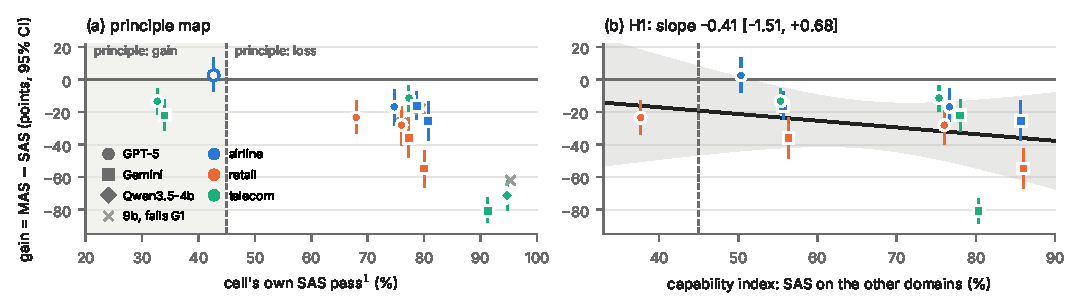
\includegraphics[width=\linewidth]{figures/fig_main.pdf}
\end{center}
\caption{(a) Principle map: each of the 13 cells' own SAS \passone\ against its gain with the paired task-cluster 95\% interval; the principle predicts a gain left of the dashed 45\% line and a loss right of it; the hollow marker is the one cell whose interval covers zero; grey crosses are the three \texttt{qwen3.5-9b} cells that fail the mechanical bars. No regression is drawn on this axis. (b) H1: the same gains against the leave-one-domain-out index for the 12 cells of the primary fit, with the weighted fit at the mean family and domain effect and its 95\% band. The two telecom cells left of 45\% in (a) move right of it. Colour marks the domain and shape the family.}
\label{fig:main}
\end{figure}

\begin{table}[t]
\caption{\textbf{The gain shows no detectable dependence on capability, and its fitted level is negative across the observed range.} Left: the H1 slope (points of gain per point of index) under each form; the primary form carries the test (minimum detectable slope in our power analysis $0.20$). $^{a}$Other units. Right: the primary fit at the mean family and domain effect.}
\label{tab:h1}
\begin{center}
\scriptsize
\setlength{\tabcolsep}{4pt}
\begin{minipage}[t]{0.60\linewidth}
\centering
\setlength{\tabcolsep}{3pt}
\begin{tabular}{@{}lccc@{}}
\toprule
Form & Cells & Slope [95\% CI] & Perm.\ $p$ \\
\midrule
leave-one-domain-out index (primary) & 12 & $-0.41$ [$-1.51$, $+0.68$] & 0.43 \\
split seeds & 12 & $-0.44$ [$-0.95$, $+0.07$] & -- \\
logit gain$^{a}$ & 12 & $-1.61$ [$-4.96$, $+1.75$] & -- \\
relative gain$^{a}$ & 12 & $-0.35$ [$-1.40$, $+0.70$] & -- \\
primary with the \texttt{qwen3.5-9b} cells & 15 & $-0.28$ [$-1.26$, $+0.69$] & 0.59 \\
own SAS score (naive, biased) & 12 & $-0.55$ [$-1.16$, $+0.06$] & -- \\
\bottomrule
\end{tabular}
\end{minipage}\hfill
\begin{minipage}[t]{0.37\linewidth}
\centering
\begin{tabular}{@{}lc@{}}
\toprule
Index & Fitted gain [95\% CI] \\
\midrule
37.7\% (lowest cell) & $-16$ [$-50$, $+18$] \\
45\% & $-19$ [$-46$, $+8$] \\
60\% & $-25$ [$-41$, $-9$] \\
86\% (highest cell) & $-36$ [$-62$, $-10$] \\
\midrule
weighted mean, 12 cells & $-28$ [$-44$, $-12$] \\
\bottomrule
\end{tabular}
\end{minipage}
\end{center}
\end{table}

Table~\ref{tab:h1} and Figure~\ref{fig:main}b give the primary test. On the 12 cells with a leave-one-domain-out index (two families, two tiers, three domains; 7 residual degrees of freedom) the slope of gain on the index is $-0.41$ (95\% CI $[-1.51, +0.68]$; permutation $p = 0.43$ two-sided, $0.21$ one-sided), so H1 is not supported and, by our reading rule, the fitted line has no crossing. Every other form agrees in sign and detects no slope, including the naive form, which is biased toward one. No family-by-index interaction is detected (CI $[-3.07, +1.58]$).

This null cannot be read as $|\beta| < 0.20$, the bound our power analysis targeted. The cells scatter around the line far more than task sampling allows: the weighted residual variance is 18.6 times its sampling expectation. What the data do fix is the level: the fitted gain is negative across the observed index range and its interval excludes zero from 60\% upward. The index also relocates the two cells the principle is distinctive about (Table~\ref{tab:rule}, index 78.0 and 55.3\%), so their low scores are a domain effect. The one cell whose index falls below 45\%, retail $\times$ \texttt{gpt-5-nano} (37.7\%), loses 23.3 points.

\subsection{H2: what coordination changes about failure}
\label{sec:h4}

\begin{table}[t]
\caption{\textbf{The MAS does not detectably reduce wrongful writes and converts other failures into exhaustion and inaction.} Pooled over the 13 cells (1,950 episodes per system); paired change per episode in points, cell-cluster bootstrap CI; classes assigned in the order WW, BX, IN, other. FP (airline only; 600 episodes per system) counts judge flags among passes; ``all flags'' adds omission flags, which were not adjudicated by hand, and is an upper bound.}
\label{tab:h4}
\begin{center}
\scriptsize
\setlength{\tabcolsep}{4pt}
\begin{tabular}{@{}lcccc@{}}
\toprule
Outcome & SAS & MAS & Change per episode [95\% CI] & Cells down / up \\
\midrule
pass & 1,362 & 768 & $-30.5$ [$-43.6$, $-18.6$] & 12 / 1 \\
wrongful write (WW) & 55 & 43 & $-0.6$ [$-2.6$, $+1.2$] & 5 / 5 \\
budget exhausted (BX) & 0 & 666 & $+34.2$ [$+24.5$, $+44.3$] & 0 / 13 \\
inaction (IN) & 126 & 268 & $+7.3$ [$+3.7$, $+11.8$] & 1 / 10 \\
other failure & 407 & 205 & $-10.4$ [$-17.0$, $-4.3$] & 10 / 3 \\
\midrule
FP, commission (airline) & 27 of 415 passes & 17 of 332 passes & $-1.7$ (4 clusters, no CI) & 4 / 0 \\
FP, all flags (airline) & 58 of 415 passes & 57 of 332 passes & $-0.2$ (4 clusters, no CI) & 2 / 2 \\
\bottomrule
\end{tabular}
\end{center}
\end{table}

A wrongful write is possible only where the gold trajectory has no write: 24 of 50 tasks on airline, 16 on telecom, 3 on retail. H2a fails on its wrongful-write half: across the 12 SAS cells WW/failures does not decline with the index (slope $-0.15$, 95\% CI $[-0.64, +0.34]$, permutation $p = 0.78$); the rate is high only for \texttt{gpt-5-nano} on airline (33\% of failures). Under the reading grid for H2b the MAS shows no detectable change in wrongful writes (Table~\ref{tab:h4}), so we find no evidence that the architecture acts on the failures it targets. The failures it did change lie elsewhere: exhaustion and inaction rise, and other failures fall. The one cell where the MAS halves wrongful writes, airline $\times$ \texttt{gpt-5-nano} (28 to 14), is the tie of the grid, and there inaction and exhaustion rise by 35 episodes. On airline, the judge flags a commission, an action or offer the policy forbids, in 6.5\% of SAS passes and 5.1\% of MAS passes; about half of the pooled drop follows from the 83 fewer passes of the MAS, and with omission flags included the two systems are level. Commission flags fall with capability (15.6 to 2.5\% of passes), against H2a's second half, on four cells of one domain.

\paragraph{Counts per cell.} Applying the taxonomy of \S\ref{sec:measures} to every episode of the 13 cells, with the database agent's executed calls counted as the MAS's writes, reproduces our earlier count for the gate run (2 wrongful writes among 29 failures); Table~\ref{tab:taxonomy} gives the counts per cell.

\paragraph{FP per cell.} \texttt{nl\_screen.py} ran the benchmark's own assertion judge (\texttt{gpt-4.1}, temperature 0) on every passing episode of the four airline cells, \Sone\ and \Mone, on 26 September; the gate run's earlier screen supplies airline $\times$ \texttt{gemini-3-flash} \Sone. Of 31 distinct unmet assertions, those whose text begins ``Agent does not / should not / must not / should never / never / should refuse'' are commission-type and count as FP as-is; the rest (duties to detect, verify, identify or communicate) are omission-type and enter only after hand adjudication, which has not been done, so the all-flags count is an upper bound. Per cell, commission / all flags among passes: \texttt{gpt-5-nano} 10 / 20 of 64 (\Sone) and 9 / 22 of 68 (\Mone); \texttt{gemini-3.1-flash-lite} 6 / 12 of 118 and 1 / 10 of 94; \texttt{gpt-5-mini} 8 / 14 of 112 and 6 / 17 of 87; \texttt{gemini-3-flash} 3 / 12 of 121 and 1 / 8 of 83. Pooled change per episode, commission $-1.7$ points and all flags $-0.2$ points; with four clusters no interval is reliable, and part of the commission drop reflects the MAS's fewer passes.

\begin{table}[tbp]
\caption{Failure taxonomy per cell meeting the mechanical bars (episodes out of 150): passes, wrongful writes, budget exhausted, inaction, other.}
\label{tab:taxonomy}
\begin{center}
\scriptsize
\setlength{\tabcolsep}{4pt}
\begin{tabular}{@{}llrrrrrcrrrrr@{}}
\toprule
 & & \multicolumn{5}{c}{\Sone} & & \multicolumn{5}{c}{\Mone} \\
\cmidrule{3-7}\cmidrule{9-13}
Model & Domain & PASS & WW & BX & IN & OTHER & & PASS & WW & BX & IN & OTHER \\
\midrule
\texttt{gpt-5-nano} & airline & 64 & 28 & 0 & 10 & 48 & & 68 & 14 & 23 & 22 & 23 \\
 & retail & 102 & 0 & 0 & 16 & 32 & & 67 & 0 & 22 & 23 & 38 \\
 & telecom & 49 & 12 & 0 & 8 & 81 & & 29 & 5 & 19 & 51 & 46 \\
\texttt{gpt-5-mini} & airline & 112 & 5 & 0 & 12 & 21 & & 87 & 0 & 31 & 24 & 8 \\
 & retail & 114 & 0 & 0 & 8 & 28 & & 72 & 0 & 51 & 17 & 10 \\
 & telecom & 116 & 1 & 0 & 10 & 23 & & 99 & 2 & 24 & 10 & 15 \\
\texttt{gemini-3.1-flash-lite} & airline & 118 & 0 & 0 & 13 & 19 & & 94 & 1 & 39 & 12 & 4 \\
 & retail & 116 & 1 & 0 & 10 & 23 & & 62 & 0 & 72 & 10 & 6 \\
 & telecom & 51 & 0 & 0 & 18 & 81 & & 18 & 5 & 62 & 42 & 23 \\
\texttt{gemini-3-flash} & airline & 121 & 2 & 0 & 11 & 16 & & 83 & 0 & 48 & 17 & 2 \\
 & retail & 120 & 0 & 0 & 8 & 22 & & 38 & 0 & 94 & 16 & 2 \\
 & telecom & 137 & 2 & 0 & 2 & 9 & & 16 & 11 & 95 & 17 & 11 \\
\texttt{qwen3.5-4b} & telecom & 142 & 4 & 0 & 0 & 4 & & 35 & 5 & 86 & 7 & 17 \\
\midrule
Total & & 1362 & 55 & 0 & 126 & 407 & & 768 & 43 & 666 & 268 & 205 \\
\bottomrule
\end{tabular}
\end{center}
\end{table}

\subsection{Robustness, sensitivity and deployment cost}
\label{sec:robust}

R1 re-ran both \texttt{gemini-3.1-flash-lite} cells at $1\times$ with the SAS capped too. Capping the SAS at its own 75th percentile costs it 4.0 and 6.7 points (telecom, airline), which sizes the asymmetry of \S\ref{sec:budget}. The gain is negative at both budgets ($-27.3$ and $-24.0$ at $1\times$, $-22.0$ and $-16.0$ at $4\times$), and its change between them has an interval covering zero on both cells (Appendix~\ref{app:card}), so no budget dependence is claimed; the larger budget cuts exhausted MAS episodes from 98\% to 45 and 31\% and lifts the MAS by 9 to 15 points, without closing the gap. R2 re-ran three airline cells with the benchmark's default simulator, \texttt{gpt-4.1}. On the two Gemini cells the gain barely moves (\texttt{gemini-3.1-flash-lite} $-19.3$ against $-16.0$, change $-3.3$, CI $[-11.3, +6.0]$; \texttt{gemini-3-flash} $-29.3$ against $-25.3$, change $-4.0$, CI $[-10.7, +2.7]$). On \texttt{gpt-5-nano}, the straddling cell, the SAS falls to 37.3\% (CI $[30.0, 45.3]$) and the MAS gains $+10.0$ (CI $[+1.3, +19.3]$), the only gain interval above zero in the study; the change between simulators, $+7.3$ (CI $[-3.3, +18.0]$), covers zero, and it is one contrast among many with no multiplicity adjustment. In dollars the MAS costs 1.4 to 3.1 times the SAS per cell (2.3 to 4.0 times for the agent calls alone), and the SAS is more accurate and cheaper in 11 of the 12 priced cells, all but the straddling cell (Table~\ref{tab:costs}). The strong SAS, which separates a loss from dividing the work from a loss from the scaffolding, is reported next (\S\ref{sec:extension}).

\subsection{Extension: the strong SAS}
\label{sec:extension}
\label{app:extension}

S2, the strong SAS: one agent, one model, one context; every call sees the conversation as the SAS does under the base prompt plus one role block. Each turn is two calls. \emph{Plan} (tools shown with \texttt{tool\_choice} ``none'') returns a JSON update of a task ledger and a progress ledger, a policy check (the applicable policy lines quoted and what they require) and a draft of the next action; \emph{act} (native tools) reviews the draft against the policy check and the conversation, revises it if needed, and acts. Budget identical to the MAS cell of the same model and domain ($4\Bx$, $c = \Bx$, $w$, $a_{\min}$, the same status line and notice); after the wrap-up notice a turn is one call without tools and without a plan, as in the SAS; an unparsable plan is retried once; an act reply that is JSON text is never sent (a message drafted inside it is used, else the act call is repeated once with a reminder). Comparators: the SAS is the calibration run, the MAS the $4\times$ grid cell, both reused. Outcomes per cell: $\Mone - \text{S2}$ and $\text{S2} - \Sone$ with task-cluster CIs, completion tokens and the S2/\Sone\ ratio, exhaustion and utilisation, review outcomes (kept, revised, replaced), and the mechanical bars. Reading: (1) $\text{S2} - \Sone$ with a CI below zero on a cell means plan-and-review scaffolding inside one context also loses at the same ceiling, so the grid loss there is not specific to dividing the work among agents; (2) $\text{S2} - \Sone$ covering zero or above it while $\Mone - \text{S2}$ lies below zero attributes the loss to the division; (3) any other pattern is reported as mixed. The first smoke (5 tasks $\times$ 1 trial per cell) passed every mechanical bar; three problems were fixed before the full run, after a second smoke round that also passed every bar (JSON act replies reaching a closing call; plans whose draft was a narrative of the plan where the next action belonged, fixed by one sentence in the block; a logging artefact), with reward read last and playing no part. Cost stop \$75. M2 (Figure~\ref{fig:design}b), in which the policy advisor becomes a checker that can veto an order or a customer message, is outlined but not evaluated here. One confound is stated at the outset: S2's plan call sees the tool definitions and the MAS orchestrator does not, so $\Mone - \text{S2}$ measures the division of work together with schema visibility, and the smoke of the fix (\S\ref{sec:compliance}) shows that schema visibility alone moves the share of write orders executed as issued from about 25\% to 72\%.

\paragraph{Results.} Telecom $\times$ \texttt{gemini-3.1-flash-lite} (150 episodes, no infrastructure errors, \$14.04): S2 36.0\% $[28.8, 43.9]$ against 34.0\% for the SAS and 12.0\% for the MAS at $4\times$; per task against the SAS, better on 15, equal on 23 and worse on 12. S2 exhausted 39 of 150 episodes (the MAS 67); its finished episodes passed 54 of 111 and its exhausted ones none. Its median completion tokens per episode were 5.4 times the SAS's (the MAS 5.8). The mechanical bars pass: 33 of 3,664 calls were cut at $c$, all act calls followed by a closing call, and no JSON or cut text reached the customer. Of 39 act replies that came back as JSON, 22 carried a usable message, 38 were repeated once, and 6 repeats that were JSON again became the holding line (6 of 855 customer messages). Over 1,807 turns the review kept the draft 779 times, revised arguments 135 times, changed the tool 419 times (the model drafts tool names that do not exist), reworded the message 306 times and changed the action type 62 times. Reading (2) holds: the loss on this cell comes from dividing the work among agents, or from the schemas the division withheld from the planner. Read with the uncapped arm for the same cell, where the MAS ties the SAS, what the division costs here is budget spent on coordination: under the same ceiling and a similar spend ratio, the single context finishes more episodes and passes more of those it finishes. $\text{S2}-\Sone$ carries the asymmetry of an uncapped SAS comparator.

Airline $\times$ \texttt{gpt-5-nano}, the straddling cell (150 episodes, no infrastructure errors, \$11.30): S2 45.3\% $[37.6, 53.3]$ against 42.7\% for the SAS and 45.3\% for the MAS at $4\times$; per task against the SAS, better on 12, equal on 27 and worse on 11. S2 exhausted 37 of 150 episodes (the MAS 35); its finished episodes passed 58 of 113 and its exhausted ones 10 of 37. Its median completion tokens per episode were 4.9 times the SAS's (the MAS 2.9). The mechanical bars pass: 20 of 3,076 calls were cut at $c$, and no JSON or cut text reached the customer; 18 of 692 customer messages were the holding line. Neither reading (1) nor reading (2) holds ($\text{S2}-\Sone$ $+2.7$ $[-5.3, +11.3]$; $\Mone-\text{S2}$ $0.0$ $[-8.7, +8.7]$), so the cell is mixed: the three systems tie.

Telecom $\times$ \texttt{gpt-5-nano}, the other cell below 45\% (150 episodes, no infrastructure errors, \$20.14): S2 27.3\% $[20.8, 35.0]$ against 32.7\% for the SAS and 19.3\% for the MAS at $4\times$; per task against the SAS, better on 7, equal on 29 and worse on 14. S2 exhausted 64 of 150 episodes (the MAS 23); its finished episodes passed 40 of 86 and its exhausted ones 1 of 64. Its median completion tokens per episode were 4.9 times the SAS's (the MAS 2.8). Split by episode ending, each episode scored against the SAS on the same task, exhausted episodes carry $-8.0$ $[-12.0, -4.2]$ points and finished ones $+2.7$ $[-2.7, +8.2]$, so the shortfall of S2 runs through the budget. The mechanical bars pass: 46 of 6,193 calls were cut at $c$, and no JSON or cut text reached the customer; 58 of 903 customer messages (6.4\%) were the holding line. Reading (1) does not hold ($\text{S2}-\Sone$ $-5.3$ $[-12.7, +1.3]$) and reading (2) holds ($\Mone-\text{S2}$ $-8.0$ $[-14.7, -1.3]$). Across the three cells, S2 does not differ detectably from the SAS, and the MAS loses to S2 on both cells below 45\%.

\subsection{Compute and cost}
\label{sec:compute}
\label{app:compute}

Episodes reported, 7,950 in all: the 16 SAS and 16 MAS grid cells (4,800); the October-build retail \texttt{qwen3.5-4b} SAS and MAS (300); three uncapped MAS cells (450); two MAS cells at $r = 25$ (300); R1, a capped SAS and a $1\times$ MAS on two cells (600); R2, SAS and MAS on three airline cells with the second simulator (900); S2 on three cells (450); and a duplicate retail $\times$ \texttt{qwen3.5-9b} MAS run (150). Pilots and smoke runs are not counted. Commercial API spend recorded by the runner (agent plus simulator at list prices): six Gemini MAS cells about \$88 and their \Sone\ cells about \$43; six GPT-5 MAS cells about \$112 and their \Sone\ cells about \$50; the $r = 25$ check \$39; the uncapped arm \$44.13; the two hosted 9b MAS cells \$8.48; the simulator for the local 4b telecom cells \$9.25 and for the October-build retail pair \$4.37; R1 \$17.23; R2 \$53.76; S2 \$45.48 and its smoke \$1.59; about \$516 in all. The judge pass, the seed replay (no simulator) and the collaborator's runs are not included. Table~\ref{tab:costs} gives the recorded cost per cell.

\begin{table}[tbp]
\caption{Recorded cost per cell in USD at list prices (agent plus simulator; tau2's own cost field). Ratio: MAS over SAS; agent only: the same ratio without the simulator. The local 4-billion model has no per-call price, so its cells show the simulator cost only.}
\label{tab:costs}
\begin{center}
\scriptsize
\begin{tabular}{@{}llrrrr@{}}
\toprule
Model & Domain & \Sone & \Mone\ at $4\times$ & Ratio & Agent only \\
\midrule
\texttt{gpt-5-nano} & airline & 4.66 & 9.15 & 2.0 & 2.9 \\
 & retail & 3.74 & 7.49 & 2.0 & 3.1 \\
 & telecom & 8.71 & 12.57 & 1.4 & 2.5 \\
\texttt{gpt-5-mini} & airline & 8.77 & 27.54 & 3.1 & 3.9 \\
 & retail & 6.82 & 20.83 & 3.1 & 4.0 \\
 & telecom & 16.94 & 34.45 & 2.0 & 3.4 \\
\texttt{gemini-3.1-flash-lite} & airline & 4.53 & 8.10 & 1.8 & 2.3 \\
 & retail & 4.21 & 7.37 & 1.8 & 2.3 \\
 & telecom & 5.53 & 9.53 & 1.7 & 2.6 \\
\texttt{gemini-3-flash} & airline & 8.52 & 19.43 & 2.3 & 2.6 \\
 & retail & 6.36 & 14.01 & 2.2 & 2.7 \\
 & telecom & 14.29 & 29.47 & 2.1 & 2.9 \\
\texttt{qwen3.5-4b} (simulator only) & telecom & 5.09 & 4.16 & -- & -- \\
\texttt{qwen3.5-4b} (Oct.\ build, simulator only) & retail & 2.10 & 2.27 & -- & -- \\
\texttt{qwen3.5-9b} & retail & -- & 3.28 & -- & -- \\
 & telecom & -- & 5.20 & -- & -- \\
\bottomrule
\end{tabular}
\end{center}
\end{table}

The 4-billion model ran on one laptop (Apple M4 Pro, 48 GB): on telecom, 150 \Sone\ episodes at about 2.3 minutes each and 150 MAS episodes in about 30 hours at one request at a time; on retail (October build), the \Sone\ took about 47 hours of wall time on a laptop shared with other work and the MAS about 25 hours. The seed replay took 86 minutes of model time.
